\section{Reuse and Warmstarting Optimizations}\label{sec-reuse-and-warmstarting}
After constructing the Experiment Graph and materializing its artifacts, our collaborative optimizer looks for opportunities to reuse existing materialized artifacts of the Experiment Graph and warmstart model training operations.
Every artifact of the incoming workload DAG is in one of the three following states: (1) the artifact does not exist in the Experiment Graph, (2) the artifact exists in the Experiment Graph but is unmaterialized, and (3) the artifact is materialized.
For the first two states, the client must execute the operations of the workload DAG to compute the artifact.
However, when the artifact is materialized, we can either load it from the Experiment Graph or let the client execute the operations to compute the artifact.
Both loading and computing an artifact incur costs.
In this section, we first describe our reuse algorithm, which selects a subset of the materialized artifacts, and outputs an optimized DAG with the lowest execution time, i.e., the sum of loading and computing cost of all the artifacts of the workload DAG.
Then, we discuss our model warmstarting approach for model training operations with different hyperparameters.

\subsection{Reuse Algorithm} 
\textbf{Preliminaries and Notations.} 
We refer to the workload DAG as $G_W$.
Every vertex, $v \in G_W$, has a load cost (i.e., $C_l(v)$ defined in Section \ref{sec-materialization}).
We also define $C_i(v)$ as the computation cost (in seconds) of $v$ given its input vertices (i.e., the parents of the vertex $v$) in $G_W$.
If an artifact exist in $G_E$ but is not materialized, then we set $C_l(v)=\infty$.
For artifacts that do not exist in $G_E$, $C_l(v)$ and $C_i(v)$ are also set to $\infty$.
Such artifacts have never appeared in any previous workloads; thus, Experiment Graph has no prior information about them.
Lastly, if an artifact is already computed inside $G_W$, such as the source artifacts or pre-computed artifacts in interactive workloads, we set $C_i(v)=0$, this is because the artifact is already available in the client's memory.

\textbf{Linear-time Algorithm.}
Our reuse algorithm comprises two parts: forward-pass and backward-pass.
In forward-pass, the algorithm selects the set of materialized vertices to load from the Experiment Graph into the workload DAG.
The backward-pass prunes any unnecessary materialized vertices before transferring the optimized DAG to the client.

Algorithm \ref{forward-pass} shows the details of forward-pass.
For every vertex of $G_W$, we define the recreation cost as the total cost of computing the vertex from the sources.
We store the recreation costs of the vertices in the $recreation\_cost$ dictionary.
In collaborative environments, the client always loads the source artifacts completely.
Therefore, we set their recreation cost to 0 (Lines 1 and 2).
Then, we visit every vertex in their topological order.
If the client has already computed a vertex inside $G_W$, then we set its recreation cost to 0 (Lines 5 and 6).
Otherwise, we compute the execution cost of a vertex as the sum of the compute cost of the vertex and the recreation cost of its parents (Lines 8 and 9).
We then compare the load cost of the vertex with the execution cost and set its recreation cost to the smaller of the two (Lines 10-14).
When the load cost is smaller, the algorithm adds the vertex to the set of reuse vertices.
Note that vertices that are not materialized have a load cost of $\infty$; therefore, the algorithm never loads an unmaterialized vertex.

\begin{algorithm}[h]
\KwData {$G_W$ workload DAG, $G_E$ experiment graph}
\KwResult {$\mathcal{R}$ set of vertices for reuse}
\For {$s \in sources(G_W)$}{
	$recreation\_cost[s] \coloneqq 0$\;
}
$\mathcal{R} \coloneqq \emptyset$\;
\For {$v \leftarrow topological\_order(G_W)$}{
	\eIf{$v$ computed in $G_W$}{
		$recreation\_cost[v] \coloneqq 0$\; 		
		}{
		$p\_costs \coloneqq \sum\limits_{p \in parents(v)} recreation\_cost[p] $\;
		$execution\_cost \coloneqq C_i(v) + p\_costs$\;
		\eIf {$ C_l(v) < execution\_cost$}{
			$recreation\_cost[v] \coloneqq C_l(v)$\;
			$\mathcal{R} \coloneqq \mathcal{R} \cup v$\;
		}{
			$recreation\_cost[v] \coloneqq execution\_cost$\;
		}
	}
}
return $\mathcal{R}$\;
\caption{Forward-pass}\label{forward-pass}
\end{algorithm}
After forward-pass, we must prune the set of reuse vertices to remove any artifact that is not part of the execution path.
A vertex $v \in \mathcal{R}$ is not part of the execution path if there exists at least another vertex $v' \in \mathcal{R}$ in every outgoing path starting at $v$.
Algorithm \ref{backward-pass} shows the details of the backward-pass algorithm.
In backward-pass, we visit every vertex of $G_W$ starting from the terminal vertices.
For every vertex, if it belongs to the reuse set, we add it to the final solution set ($\mathcal{R}_p$) and stop traversing its parents (Lines 4 and 5).
Otherwise, we continue traversing the parents of the vertex (Line 7).

\begin{algorithm}[h]
\KwData {$\mathcal{R}$: Current reuse set, $G_W$: workload DAG}
\KwResult {$\mathcal{R}_p$: Final reuse set after pruning}
$\mathcal{R}_p \coloneqq \emptyset$\;
$v\_queue \coloneqq terminals(G_W)$\;
\While{$v \leftarrow v\_queue.next()$}{
	\eIf{$v \in \mathcal{R}$}{
			$\mathcal{R}_p \coloneqq \mathcal{R}_p \cup v$\;
	}{
		$v\_queue.add(parents(v))$\;
	}
}
return $\mathcal{R}_p$\;
\caption{Backward-pass}\label{backward-pass}
\end{algorithm}

Figure \ref{fig-reuse-algorithm} shows how our reuse algorithm (forward-pass and backward-pass) operates on an example workload DAG.
There are 3 source vertices in the workload DAG.
The algorithm starts with forward-pass, traversing the graph from the sources (Scenario \textcircled{\raisebox{-0.9pt}{\textbf{1}}}).
For materialized vertices with a larger load cost than execution cost (i.e., the sum of the compute cost and parent's recreation costs), the algorithm sets the recreation cost to the execution cost (Scenario \textcircled{\raisebox{-0.9pt}{\textbf{2}}}).
For vertices that exist in EG but are unmaterialized, the algorithm chooses to compute them (Scenario \textcircled{\raisebox{-0.9pt}{\textbf{3}}}).
If a vertex is already computed inside the workload DAG, then the algorithm sets its recreation cost to zero (Scenario \textcircled{\raisebox{-0.9pt}{\textbf{4}}}).
For materialized vertices, which have a smaller load cost than the execution cost, the algorithm sets the recreation cost to the load cost of the vertex (Scenario \textcircled{\raisebox{-0.9pt}{\textbf{5}}}).
For example, for the materialized vertex with label $v_2$, the total execution cost is $2 + 5 + 10 = 17$, which is larger than its load cost of $16$.
Once the traversal reaches a node that does not exist in EG, the forward-pass stops (Scenario \textcircled{\raisebox{-0.9pt}{\textbf{6}}}).
At this stage, forward-pass has selected the materialized vertices $v_2$ and $v_3$ for reuse.
Then, the algorithm starts backward-pass from the terminal vertex (Scenario \textcircled{\raisebox{-0.9pt}{\textbf{7}}}).
Once the backward-pass visits a materialized vertex, it stops traversing its parents.
The backward-pass removes any materialized vertices that it did not visit (Scenario \textcircled{\raisebox{-0.9pt}{\textbf{8}}}).
For example, since $v_3$ is materialized, backward-pass stops visiting its parents; thus, it removes $v_2$ from the final solution.

\begin{figure}
\centering
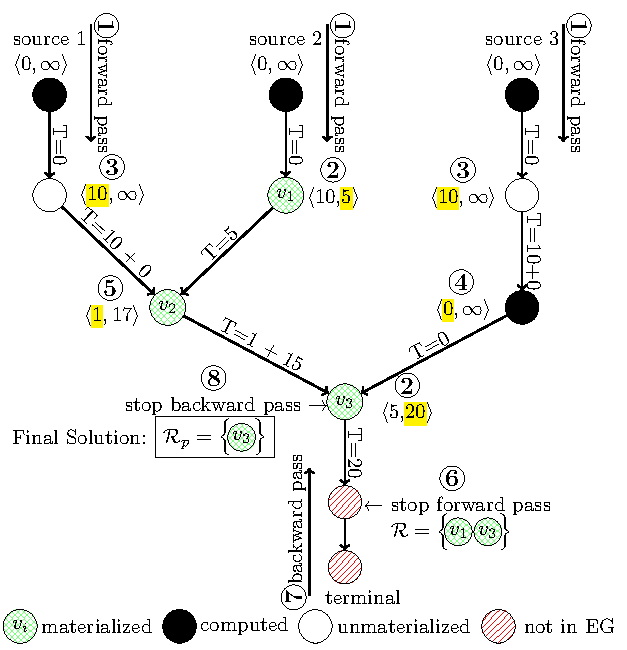
\includegraphics[width=\linewidth]{../images/tikz-standalone/reuse-algorithm}
\caption{Reuse Algorithm Example. Each vertex has the label $\langle C_i(v),C_l(v) \rangle$. $T$ represent the recreation cost passed along to the children vertices. Numbered circles show different scenarios.}
\label{fig-reuse-algorithm}
\end{figure}

\textbf{Complexity.} 
Both forward-pass and backward-pass traverse the workload DAG once, resulting in $2*|V|$ vertex visits, where $V$ is the set of vertices in the workload DAG.
Therefore, our reuse algorithm has a worst-case complexity of $\mathcal{O}(|V|)$.
However, the number of vertex visits in each pass is smaller than $|V|$ because of the early-stopping conditions in forward and backward passes.
Backward-pass stops traversing the parents of a vertex when the vertex is in the reuse set; therefore, it does not need to visit all the vertices until it reaches the source.
Furthermore, in our implementation of forward-pass, we also include an early-stopping condition.
The early-stopping condition instructs forward-pass to stop traversing down a path when it encounters a vertex that is not in EG.
Thus, the reuse algorithm generates the optimized DAG with a small overhead.
This is an important requirement of the collaborative environments.
In a typical collaborative environment, many clients send workloads to the server for optimization.
Furthermore, in interactive workloads, clients expect a response very fast.
Therefore, If the reuse algorithm incurs a large overhead, the server does not respond in time or becomes unresponsive.

\subsection{Warmstarting}
Many model training operations include different hyperparameters, which impact the training process.
Two training operations on the same dataset with different hyperparameters may result in completely different models.
In such scenarios, we cannot reuse a materialized model in EG instead of a model artifact in the workload DAG.
Therefore, instead of reusing a model, we try to warmstart the model training operations using the models in EG.
In warmstarting, instead of randomly initializing the parameters of a model before training, we initialize the model parameters to a previously trained model.
Warmstarting has shown to decrease the total training time in some scenarios \cite{baylor2017tfx}.
Note that in many scenarios, there is no guarantee that warmstarting works.
Therefore, we only warmstart a model training operation, when users explicitly requests it.
The default behavior of our system is not to warmstart model training operations.

The process of warmstarting is as follows.
Once we encounter a model in the workload DAG in forward-pass, we check if there are candidates for warmstarting in EG.
A warmstarting candidate is a model that is trained on the same artifact and is of the same type as the model in the workload DAG.
When there is more than one candidate for warmstarting, we select the model with the highest evaluation score.
Finally, we initialize the model training operation with the selected model.